***********
This section used to be in the "Creating Variables in Opus" chapter (part-components/creating-variables.tex)

It didn't really fit there.  Is there any material that can be used for part-gui/results-manager.tex?
***********

\section{Opus Indicators}
\label{sec:opus-indicators}

Indicators are typically considered summary measures used for
evaluation purposes, like a cost-benefit ratio, or a VMT per capita
measure.  Indicators can also be used for evaluation purposes.  Opus
has a fairly extensive infrastructure for computing indicators.  Some
of it is already available in the new Opus GUI, but there is more
functionality available using scripts.  In the eugene package, for
example, there is an indicators directory containing a
make\_indicators.py script that demonstrates the use of a script to
make a series of different kinds of indicators.  
% A more extensive set
% of examples and documentation is provided in the script 
% /opus/src/opus\_core/indicator\_framework/make\_indicators\_example.py.

Indicators generally use expressions to do their computation, so they
share all of the functionality described in the preceding section.  The
Opus Indicator Framework, however, adds some very helpful methods to
also visualize the results of the indicator computation, or to export
the results to a text file, or a table in a database, or to a GIS for
visualization.

The indicator output options currently include the following types:

\squishlist 
\item \emph{Map}: produces a map of the indicator rendered
in Matplotlib. 
\item \emph{Chart}: produces a simple line chart, useful for tracking
an aggregate indicator over multiple years of a simulation. 
\item \emph{Table}: produces a browsable table that can also be
exported, containing two columns: the column containing the level of geography or
aggregation, and the column containing the indicator value for that
aggregation.  A zone table of total population would be an example of
this form. 
\item \emph{DatasetTable}: produces a table with multiple
indicators for the same unit of aggregation or geography, such as
employment by zone, with multiple columns representing the total
employment for each industry sector, and possibly other indicators.  It
would contain one record per zone. 
\squishend

The Opus GUI currently supports all these output types except the
chart. The following tutorial focuses on the use of the GUI to
create and visualize several different kinds of indicators.

Assume that we want to run the eugene\_gridcell baseline scenario from
1980 to 1990, and then will generate the following indicators from the
simulation results:

\squishlist
\item Average cars per household by gridcell, viewed as a map
\item Average cars per household by zone, viewed as a map
\item Average household size per zone, viewed as a table
\item Log of the sum of population and employment by gridcell, as a map
%\item Total population by zone, as a table
\squishend

For the first indicator, we need an expression that would compute the
average number of cars for the households living in a gridcell, and
then to display this on a map.  The expression is straightforward:

\code{cars\_per\_hh = gridcell.aggregate(household.cars, function=mean)}

Note that since we are operating on a \verb#primary attribute# of the
data (we can find \verb#cars# in the data directory under
data/eugene\_gridcell/household), we do not need to put a package name
in the expression.  We could leave out the alias \verb#cars_per_hh =#,
but when we generate the indicator and map, using an alias will provide
a meaningful default title on the Matplotlib map.

Make sure that you have run a
simulation on the computer you are using (see
Chapter~\ref{chap:scenarios-manager}) that has run over multiple
years. Create the \verb#cars_per_hh# indicator (creating a new
indicator in the GUI is covered in
Chapter~\ref{chap:variable-library}). You can visualize the result
by following the directions in
Section~\ref{sec:interrogating-results-with-indicators}. You
will see something like that shown in
figure~\ref{fig:indicator-cars-gridcell-2}.

% \begin{figure}[htp]
% \begin{center}
% 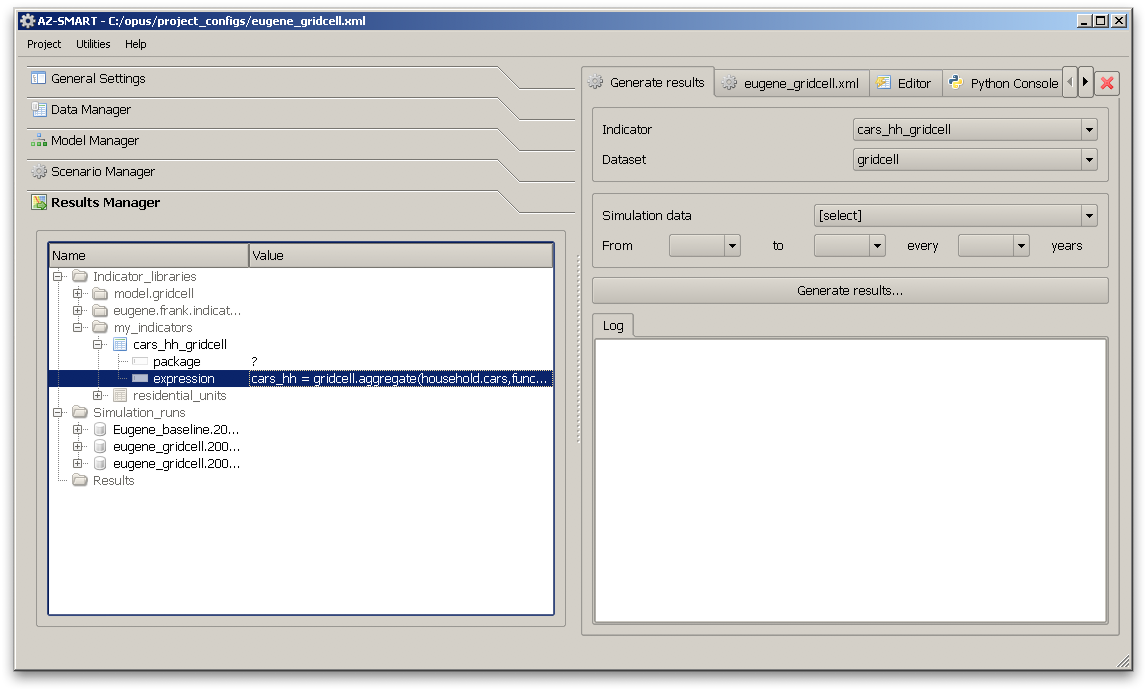
\includegraphics[scale=0.4]{graphics/indicator-cars-gridcell-1.png}
% \end{center}
% \caption{Generating the Average Cars per Household in a Gridcell}
% \label{fig:indicator-cars-gridcell-1}
% \end{figure}

\begin{figure}[htp]
\begin{center}
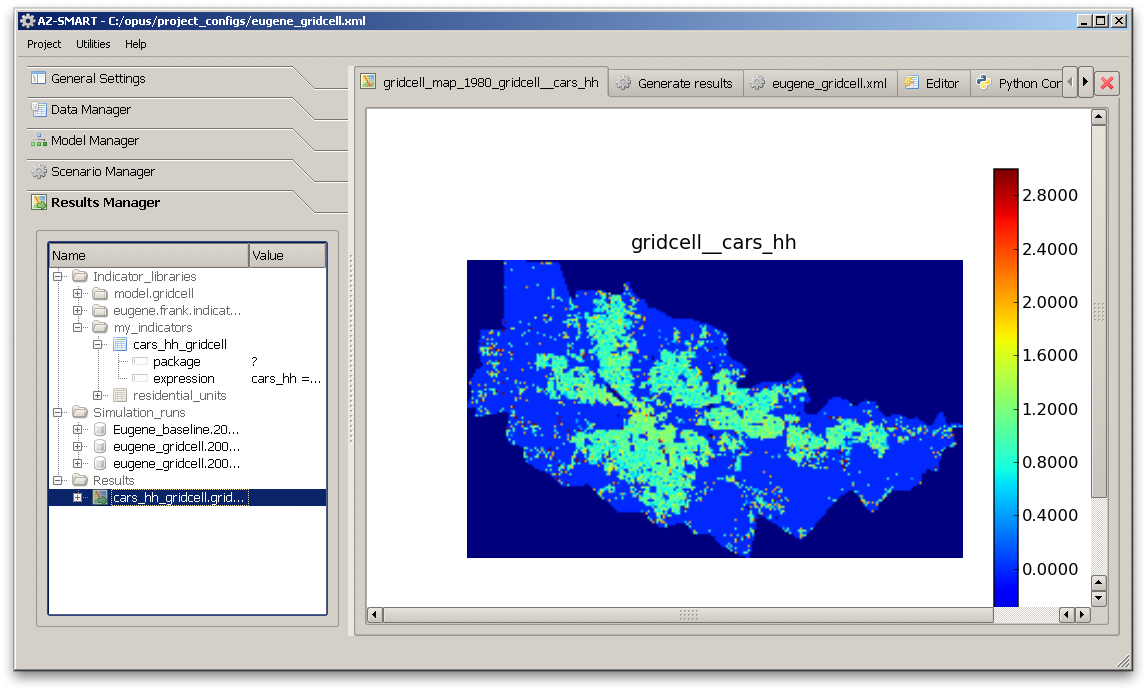
\includegraphics[scale=0.4]{graphics/indicator-cars-gridcell-2.png}
\end{center}
\caption{Generating the Average Cars per Household in a Gridcell}
\label{fig:indicator-cars-gridcell-2}
\end{figure}

In order to compute the second indicator, we will need to average the
number of cars per household at the zonal level as follows:

\code{cars\_per\_hh = zone.aggregate(household.cars, intermediates= [gridcell], function=mean)}

% T: this is actually not true, it works just fine
% The only remaining problem with this is that we cannot display zonal
% data using Matplotlib, which generates only raster image maps, meaning
% that it only supports displaying data assigned to gridcells.  Recalling
% the \verb#disaggregate# function in the expression language, we can
% just disaggregate the zonal average like this:
% 
% \code{cars\_per\_hh = gridcell.disaggregate(zone.aggregate(household.cars, intermediates= [gridcell], function=mean))}

To generate the third indicator of average household size we could use
a similar expression:

\code{persons\_per\_hh = zone.aggregate(household.persons, function=mean, intermediates = [gridcell])}

Now we use a compound expression, to sum the result of two variables,
and take the log of the result.  This is to produce the indicator as
shown below:

\code{ln\_emp\_pop=ln(urbansim.gridcell.population+urbansim.gridcell.number\_of\_jobs)}

Note that these are variables which can be found on the disk in
src/urbansim/gridcell.  The result of visualizing this indicator is
shown in Figure \ref{fig:indicator-ln-emp-pop}.

\begin{figure}[htp]
\begin{center}
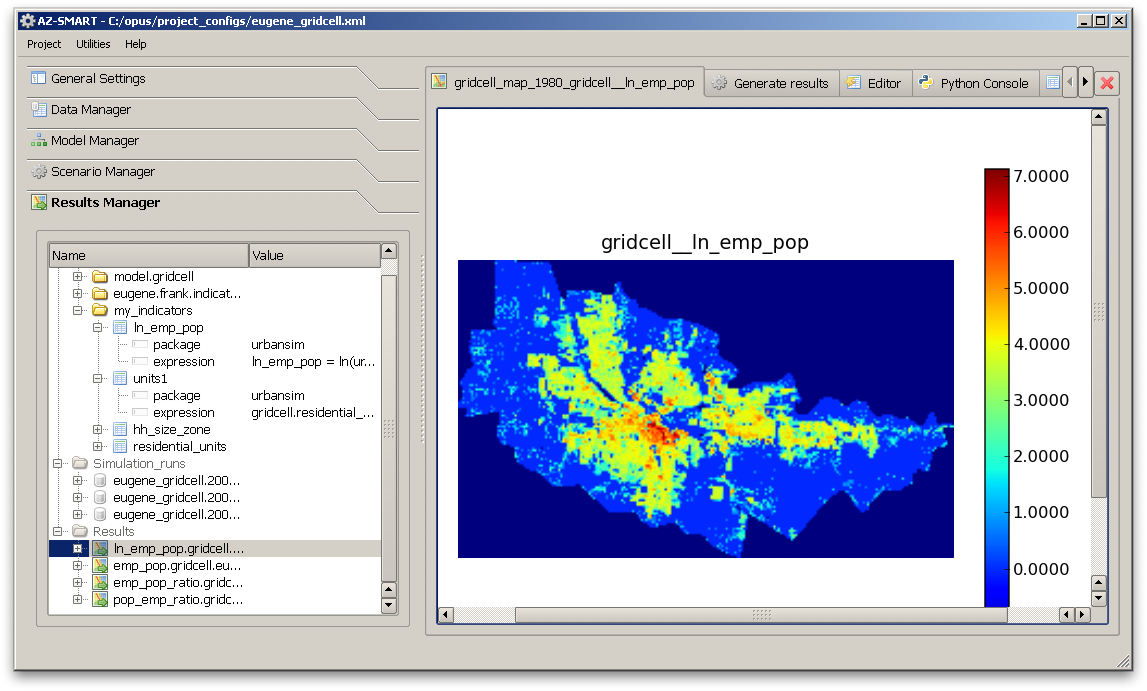
\includegraphics[scale=0.4]{graphics/indicator-ln-emp-pop.png}
\end{center}
\caption{Log of (Population + Employment) by Gridcell}
\label{fig:indicator-ln-emp-pop}
\end{figure}

% For the last indicators in the list to be done, we return to
% indicators that are already defined in a generic indicator library in
% the results manager.  To produce the population by zone indicator and
% visualize it as a table, use the following steps.  Right-click on the
% population indicators, and select \verb#Generate results with#.  In the
% form that is created on the right, select the pull-down menu labeled
% \verb#Dataset# and click on zone.  This is a generalized indicator that
% uses a simple mechanism to allow different levels of aggregation to be
% selected in this way, without the need to type in an expression as was
% done in the preceding examples.  Select a simulation result, and
% generate the indicator.  Then select the new indicator result
% containing the indicator values, right-click, and select \verb#View
% result as# and choose \verb#Table#.  This should generate a browsable
% table in the form window, as shown below in Figure
% \ref{fig:indicator-population-zone-table}.
% 
% \begin{figure}[htp]
% \begin{center}
% 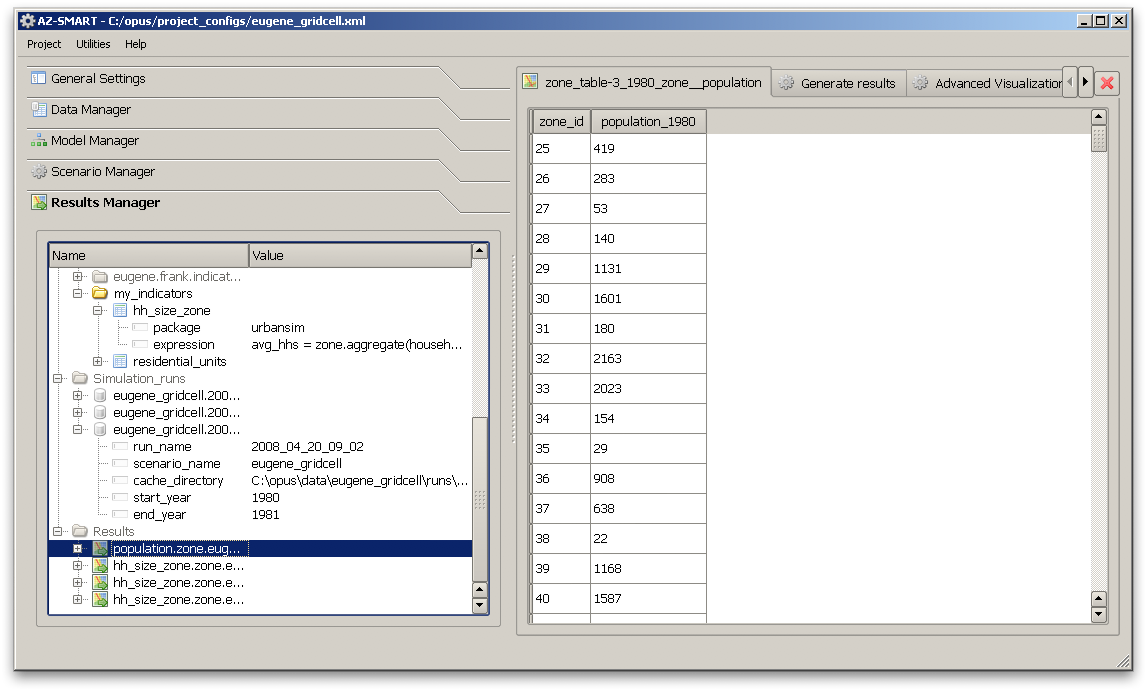
\includegraphics[scale=0.4]{graphics/indicator-population-zone-table.png}
% \end{center}
% \caption{Viewing the Population by Zone Indicator as a Table}
% \label{fig:indicator-population-zone-table}
% \end{figure}
% 
% Now that we have seen the integrated Matplotlib maps, you might want to
% know how to export an indicator to a more full-featured GIS system such
% as ArcGIS (a commercial package from Environmental Systems Research
% Institute), or PostGIS (an open source package built on the Postgres
% database).  The Results Manager is now able to export a table with one
% or more indicators to an ESRI Geodatabase for further analysis and
% visualization.  In the following example, we export the same indicator
% result shown above as a table, to an ESRI File-based Geodatabase. 
% Other Geodatabase formats are also supported.
% 
% If the population by zone table result is still available, right-click
% on the result in the tree on the left-hand side of the window, and
% select the \verb#View result as# and choose \verb#Advanced
% visualization#.  It will generate a form as shown in Figure
% \ref{fig:indicator-population-zone-export}.  We need to add the
% indicator we have generated to the set, in the upper portion of this
% form, and select the location of the ESRI geodatabase.  I am assuming
% that the geodatabase contains a \verb#Feature Class# corresponding to
% the table being exported. In this example, the table corresponds to the
% zone feature class.  Once the form is filled in, click on the
% \verb#Go!# button, to start the export process.  A message will be
% printed to the log to indicate the completion status of this export
% process.
% 
% \begin{figure}[htp]
% \begin{center}
% 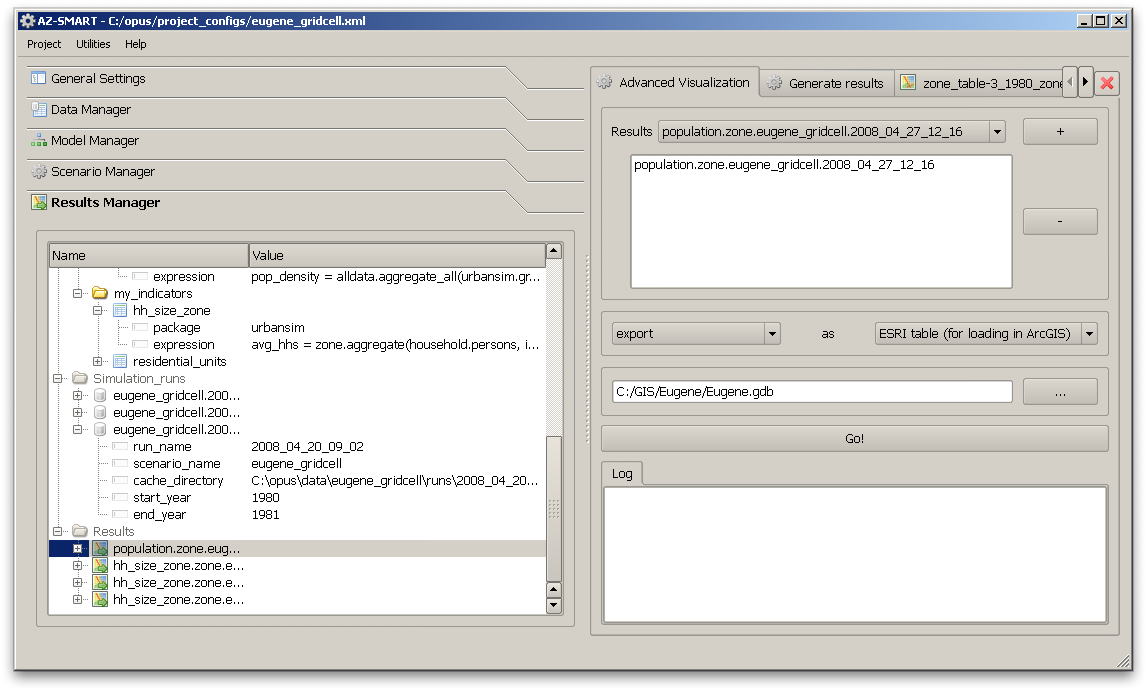
\includegraphics[scale=0.4]{graphics/indicator-population-zone-export.png}
% \end{center}
% \caption{Exporting the Population by Zone Indicator to an ESRI Geodatabase}
% \label{fig:indicator-population-zone-export}
% \end{figure}
% 
% Once the export is successfully completed, the geodatabase will contain
% a table that contains the indicator result, with a zone\_id and an
% ArcGIS \verb#OBJECTID*# that corresponds to the internal object ids in
% the feature class.  It is safe to join the indicator table result with
% the feature class using either the objectid or the zone\_id.  The map
% in Figure \ref{fig:indicator-population-zone-arcgis} shows the result
% of joining the feature class with the indicator table and generating a
% thematic map of the populaion by zone, using the zone.acres field to
% normalize the population, resulting in a map of population density per
% acre.
% 
% \begin{figure}[htp]
% \begin{center}
% 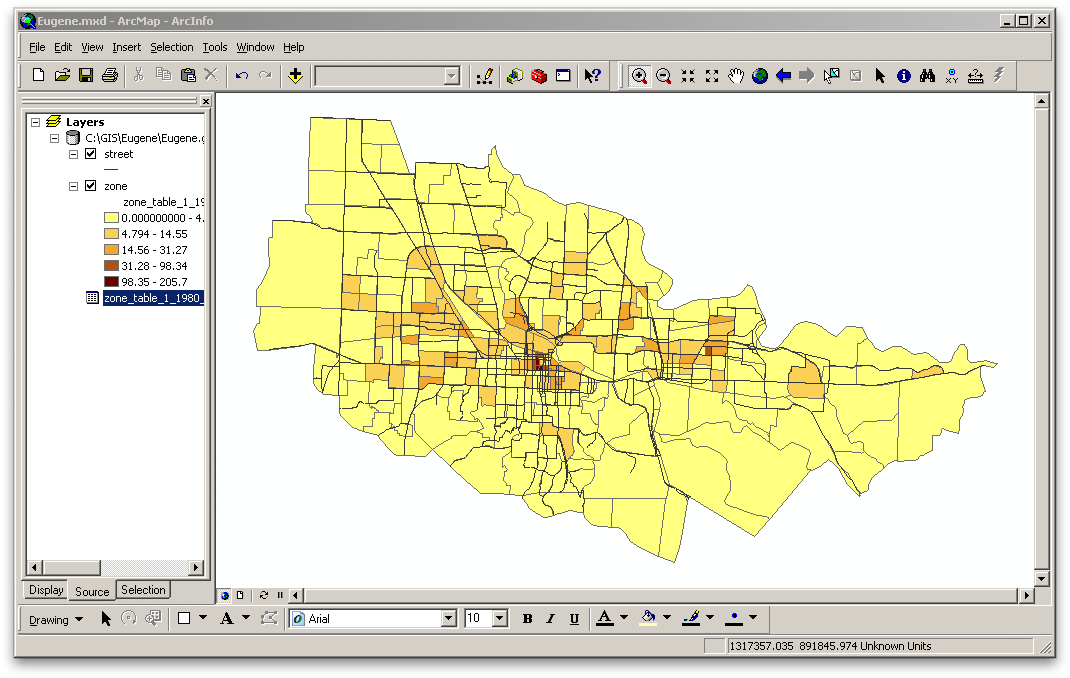
\includegraphics[scale=0.4]{graphics/indicator-population-zone-arcgis.png}
% \end{center}
% \caption{Mapping the Population by Zone Indicator in ESRI ArcMap}
% \label{fig:indicator-population-zone-arcgis}
% \end{figure}
